% Intended LaTeX compiler: pdflatex
\documentclass[10pt,article]{article}
\usepackage[utf8]{inputenc}
\usepackage[T1]{fontenc}
\usepackage{graphicx}
\usepackage{grffile}
\usepackage{longtable}
\usepackage{wrapfig}
\usepackage{rotating}
\usepackage[normalem]{ulem}
\usepackage{amsmath}
\usepackage{textcomp}
\usepackage{amssymb}
\usepackage{capt-of}
\usepackage{hyperref}
\usepackage{titling} \posttitle{\par\end{center}} \setlength{\droptitle}{-30pt} \usepackage{multicol} \setlength{\columnsep}{1cm} \usepackage[T1]{fontenc} \usepackage[utf8]{inputenc} \renewcommand{\contentsname}{Table of Contents / Agenda} \usepackage[letterpaper,left=1in,right=1in,top=0.7in,bottom=1in,headheight=23pt,includehead,includefoot,heightrounded]{geometry} \usepackage{fancyhdr} \pagestyle{fancy} \fancyhf{} \cfoot{\thepage} \usepackage{mathpazo} \usepackage[scaled=0.85]{helvet} \usepackage{courier} \usepackage[onehalfspacing]{setspace} \usepackage[framemethod=default]{mdframed} \usepackage{wrapfig} \usepackage{booktabs} \usepackage[outputdir=Lectures]{minted}
\setcounter{secnumdepth}{3}
\date{\vspace{-6ex}}
\title{Class 2: Hypothesis Testing for a Mean and Significance of Regression Coefficients}
\hypersetup{
 pdfauthor={},
 pdftitle={Class 2: Hypothesis Testing for a Mean and Significance of Regression Coefficients},
 pdfkeywords={},
 pdfsubject={Description School specific teaching materials},
 pdfcreator={Emacs 26.1 (Org mode 9.1.13)}, 
 pdflang={English}}
\begin{document}

\maketitle
\lhead{ COURSE 0000 \\ Joon H. Ro } 
\rhead{ Class 2 \\ 2018-08-30 Thu} 
\thispagestyle{fancy}

\setcounter{tocdepth}{1}
\tableofcontents
\vspace{6ex}

\section{Review: Regression and Interpretation of Regression Results}
\label{sec:orgaba09e3}
\[  y_{i} = \beta_0 + \beta_1 x_{i, 1}  + \beta_2 x_{i, 2} + \cdots +  + \beta_K x_{i, K}  \varepsilon_{i} \]

\begin{itemize}
\item Last class, we talked about how to interpret regression results
\end{itemize}

\subsection{Model Level}
\label{sec:orga34da2d}
\begin{itemize}
\item \(R^2\): How much variation in \(y\) can my model explain?

\[ R^{2} = 1 - \dfrac{SS_{error}}{SS_{total}} \]
\item We use \textbf{adjusted} \(R^2\) to compare regressions with
different numbers of independent variables
\end{itemize}

\subsection{Variable Level (Coefficients)}
\label{sec:org2f84842}
\begin{itemize}
\item How does \(x_1\) affects \(y\)?
\item \(\beta_1\): How \(y\) changes if \(x_1\) is increased by 1 unit
\end{itemize}
\subsection{Significance}
\label{sec:orgaca2597}
\begin{itemize}
\item How do we know if those coefficients are \emph{significant}?
\item Does \(x_1\) affects \(y\)?

\begin{itemize}
\item We do hypothesis testing for each of the coefficients separately
\end{itemize}
\end{itemize}
\section{Sampling Distribution and Variance of the Sample Mean}
\label{sec:org473deec}
\begin{itemize}
\item Suppose we can \emph{repeatedly} draw random samples of size \(n\) from the population
\item Then calculate the mean for \emph{each} sample:

\begin{itemize}
\item e.g., \(\bar{x}_1\): mean of the first sample, \(\bar{x}_2\): mean of
the second sample, \ldots{}
\end{itemize}

\item Computation of variance of these \uline{means}:

\(s^2_{\bar{x}} = \dfrac{s^2}{n} \begin{cases} 
       \Uparrow &  \text{increases with increasing sample variance} (s^2) \\
       \Downarrow & \text{decreases with increasing sample size} (n)
       \end{cases}\)
\end{itemize}

\subsection{How reliable is the sample mean as the sample size increases?}
\label{sec:org9d5a6c7}
\begin{itemize}
\item The histogram of \uline{sample means} will eventually look like a normal
distribution when \(n\) becomes larger and larger. (Central-Limit Theorem)
\item The histogram will also be "thinner" as \(n\) goes larger.

\begin{center}
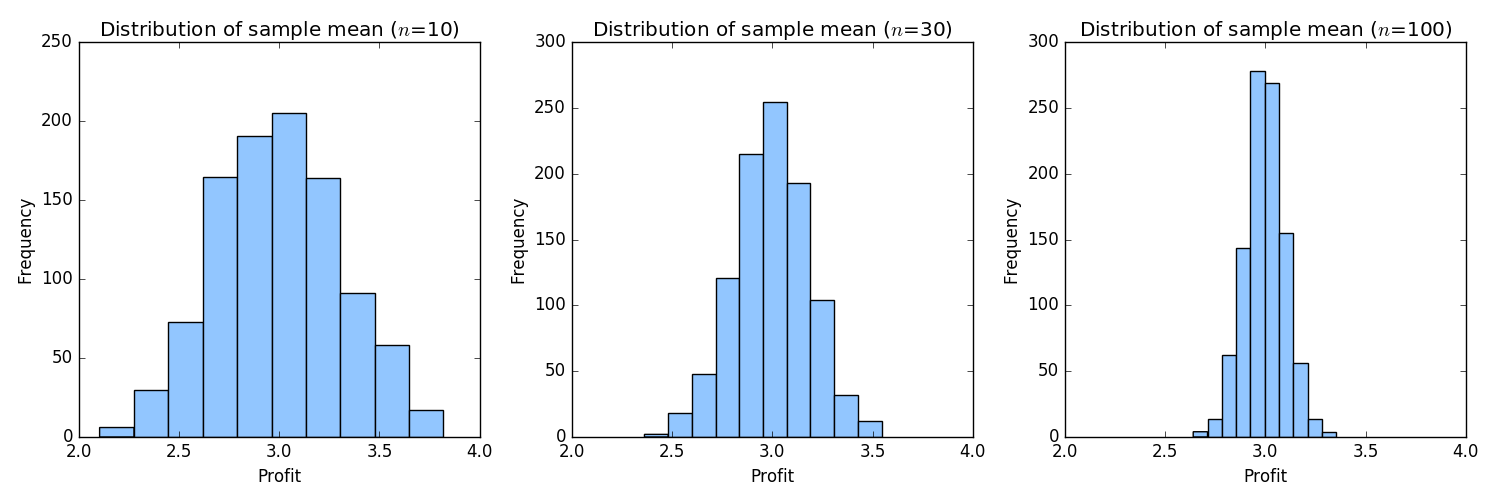
\includegraphics[width=13cm]{../../../Assets/Images/Statistics/hist_mean_n.png}
\end{center}

(these are generated with 1,000 draws of samples with size \(n\) - that
is, we have 1,000 independent samples each with \(n\) observations)
\end{itemize}

\subsection{Sample Mean and Standard Error}
\label{sec:org02dc014}
\begin{multicols}{2}
\begin{description}
\item[{Sample mean}] \(\overline{x}\)

Accuracy of sample mean depends on:
\begin{description}
\item[{Sample variance}] \(s_x^2\)
\item[{Sample size}] \(n\)
\end{description}
\end{description}

\begin{description}
\item[{Standard Error}] \(SE_{\overline{x}} = \sqrt{\dfrac{s^2_x}{n}}\)
\end{description}

\end{multicols}

\subsection{Standard Deviation VS. Standard Error}
\label{sec:orga9f4e85}
\begin{description}
\item[{Standard deviation (\(s_{x}\))}] Describes the spread of values in the sample 

\begin{itemize}
\item The sample standard deviation, \(s_x\) is a random quantity - it varies from
sample to sample
\item Becomes \textbf{more accurate representation of the population standard
deviation} when the sample size increases
\end{itemize}
\end{description}

\begin{description}
\item[{Standard error of the mean (\(SE_{\bar{x}}\))}] the standard deviation of
the sample mean \(\bar{x}\)

\begin{itemize}
\item Describes \(\bar{x}\)'s accuracy as an estimate of the population mean,
\(\mu\)
\item When the sample size increases, the estimator is based on more information
and becomes more accurate, so \textbf{its standard error decreases}
\end{itemize}
\end{description}
\subsection{Margin of error: Confidence interval of the mean}
\label{sec:org724a5c8}
\begin{itemize}
\item What is a 95\% confidence interval?
\begin{itemize}
\item If we would draw samples of the same size \uline{over and over again}, then in 95\%
of the times this interval covers the mean.
\item So it is a measure of reliability
\item \([ \bar{x}\)  \(- 1.96 SE_{\bar{x}} \), \(\quad \bar{x}\)
 \( + 1.96 SE_{\bar{x}} \) \(]\)
\end{itemize}

\item It does \uline{not} mean that "there is a 95\% chance that the population mean is
in this specific confidence interval" (See textbook page 277)
\end{itemize}
\section{Hypothesis Testing for a Mean}
\label{sec:orga21411d}
\textbf{Statements}

\begin{itemize}
\item People think that the quality of food at our restaurant is above average (5)

\item College head coaches' winning percentages affects their compensation levels
(Regression)
\end{itemize}
\subsection{Testing Hypothesis about a Single Mean}
\label{sec:orgee6fc1c}
\begin{itemize}
\item People think that the quality of food at our restaurant is above average (5)

\item Null hypothesis:
\begin{itemize}
\item There is no difference or effect 

\(H_0\): Average rating of food quality is 5 or, 
\(H_0\): \(Rating_{foodquality} = 5\)
\end{itemize}
\end{itemize}

\begin{itemize}
\item Alternative hypothesis: 

\begin{itemize}
\item That there is a difference (or an effect)
\end{itemize}

\begin{multicols}{2}

\begin{itemize}
\item Two-sided
\begin{itemize}
\item The average rating of food quality is not 5

\begin{description}
\item[{\(H_{a}\)}] \(\text{rating}_{foodquality} \ne 5\)
\end{description}

\item No discrimination of the direction of difference
\end{itemize}

\item One-sided
\begin{itemize}
\item The average rating of food quality is higher than 5
\begin{description}
\item[{\(H_{a}\)}] \(\text{rating}_{foodquality} > 5\)
\end{description}

\item Some idea of the direction of difference
\end{itemize}
\end{itemize}

\end{multicols}
\end{itemize}

\begin{itemize}
\item \(H_0\): \(rating_{foodquality} = 5\)
\item \(H_a\): \(rating_{foodquality} \ne 5 \quad \text{or} \quad
  rating_{foodquality} > 5\)
\item Average rating from 100 respondents: 6.5, Variance: 4
\item Is the difference (5 VS. 6.5) statistically significant?
\end{itemize}

\subsection{z-test vs. t-test}
\label{sec:org4bef5fa}
\begin{itemize}
\item \uline{Rule of thumb}: 
\begin{quote}
"Use a z-test when the variance of the distribution is known, otherwise use
a t-test"
\end{quote}

\item For a large sample, t-test is equivalent to a z-test

\begin{itemize}
\item Mostly fine with Regression
\end{itemize}
\end{itemize}

As \(n\) increase, the t-distribution approaches the standard normal
distribution
\subsection{Recall}
\label{sec:org6390ba5}
\begin{itemize}
\item Sample mean: \(\overline{x}\)

\item Accuracy of sample mean depends on:
\begin{itemize}
\item Sample variance: \(s_x^2\)
\item Sample size: \(n\)
\end{itemize}

\item Standard Error: \(SE_{\overline{x}} = \sqrt{\dfrac{s^2_x}{n}}\)
\end{itemize}

Hence, with the example,

\begin{itemize}
\item \(\overline{x} = 6.5, \qquad\)  \( s_x^2 = 4, \qquad\)  \( n = 100 \)
\item \(SE_{\overline{x}} = \sqrt{\dfrac{s^2_x}{n}}\)  \( = \sqrt{\dfrac{4}{100}} \)  \( = .2 \)
\end{itemize}

\subsection{Computing t-statistic}
\label{sec:orged0ab46}
\begin{itemize}
\item \(H_0: \overline{x} = \overline{x}_0 \qquad (6.5 = 5)\)
\item \( H_a: \overline{x} \ne \overline{x}_0 \quad (6.5 \ne 5) \quad
  \text{or} \quad H_a: \overline{x}>\overline{x}_0 \quad (6.5 > 5) \)

\item \(t=\dfrac{\overline{x} - \overline{x}_0}{SE_{\overline{x}}}, \qquad\)
 where \(\dfrac{\overline{x} - \overline{x}_0 = 1.5}{SE_{\overline{x}} = .2} \)  \(  \quad = 7.5 \)
\end{itemize}

\begin{itemize}
\item \(t \uparrow\) \(\Rightarrow\)  p-value \( \downarrow \)

\begin{itemize}
\item p-value: the probability of finding the observed results when \(H_{0}\) is true
\end{itemize}
\end{itemize}

\subsection{t-critical}
\label{sec:org05c30d3}
\begin{itemize}
\item How large must \(t\) be to reject the null hypothesis:
\begin{itemize}
\item \(t\) must be larger than \(t_{critical}\) (threshold)
\item Since the mean of \(t\)-distribution is zero, larger the value, smaller
the probability
\end{itemize}
\end{itemize}

\begin{itemize}
\item \(t_{critical}\) depends on:
\begin{itemize}
\item Significance level \(\alpha\) (typically \(\alpha=0.05\))
\item Degrees of freedom: total sample size-1 \(\rightarrow n-1\)
\item Whether test is one sided or two sided
\item Use \uline{t-tables}. For large \(n\), you can use normal distribution (\(z\))
\end{itemize}
\end{itemize}

\begin{multicols}{2}
\begin{itemize}
\item For two-sided test:
\begin{itemize}
\item \(t_{Critical} = t_{\alpha/2, n-1}\)
\begin{itemize}
\item For large \(n\), \(t_{0.025}=1.96\)
\end{itemize}
\item Reject the null if \(|t| > t_{Critical}\)
\item Fail to reject the null if \(|t| < t_{Critical}\)
\end{itemize}
\end{itemize}

\begin{itemize}
\item For one-sided test:
\begin{itemize}
\item \(t_{Critical} = t_{\alpha, n-1}\)
\begin{itemize}
\item For large \(n, \; t_{0.05} = 1.65\)
\end{itemize}
\item Reject the null if \(t > t_{Critical}\)
\item Fail to reject the null if \(t < t_{Critical}\)
\end{itemize}
\end{itemize}
\end{multicols}

\begin{itemize}
\item In both cases, rejecting the null means p-value \(< \alpha\)
\end{itemize}

\subsection{The conclusion is}
\label{sec:org68f50b1}
\begin{multicols}{2}
\[ H_a: rating_{foodquality} \ne 5 \]

 \( |t| = 7.5 > t_{critical}=1.96 \)  \(\Rightarrow \text{ Reject } H_0 \)





\[ H_a: rating_{foodquality} > 5 \]

 \( t = 7.5 > t_{critical}=1.65 \)  \(\Rightarrow \text{ Reject } H_0 \)
\end{multicols}
\section{Significance of Regression Coefficients}
\label{sec:orgc1db947}
\begin{itemize}
\item We do hypothesis testing for a mean for \emph{each} coefficient separately
\end{itemize}
\subsection{Null and Alternative Hypotheses}
\label{sec:org7b29ae8}
\begin{itemize}
\item The null hypothesis is that there is \emph{no} effect:
\begin{itemize}
\item \(H_{0}: \beta_{k}=0 \qquad H_{A}: \beta_k \ne 0\)
\end{itemize}
\end{itemize}

\begin{itemize}
\item Null hypothesis:
\begin{itemize}
\item \(H_0\): Winning Percentage of a head coach does not affect his
compensation
\item \(H_0\): \(\beta_{WinPercentage} = 0\)
\end{itemize}

\item Alternative hypothesis: 
\begin{itemize}
\item College head coaches' winning percentages affects their compensation levels
\item \(H_{a}\): \(\beta_{WinPercentage} \ne 0\)
\end{itemize}
\end{itemize}

\subsection{Regression Results}
\label{sec:orgb10e432}
\begin{itemize}
\item \texttt{t Stat}: \(\dfrac{\hat{\beta}_{k}}{SE_{k}}\) (because \(H_0: \beta_k=0\)): Reject the null if \(T > |1.96|\)
\end{itemize}

\begin{itemize}
\item \texttt{P-value}: the probability of observing \(\hat{\beta}_{k}\) if the null
hypothesis is true: reject the null if \texttt{P-value} \(< 0.05 (=\alpha)\)
\end{itemize}

\begin{itemize}
\item 95\% \(((1-\alpha) \times 100 \%)\) Confidence interval: will not include
0 if \(\hat{\beta}_{k}\) is significant
\end{itemize}
\end{document}